\newpage
\lecture{14}{Теорема о мажорируемой подпоследовательности. Разные виды сходимости.}

\begin{exercise}
    Пусть $f_n\to f$ в $L^1$ (то есть в среднем).
    Существует ли $g\in L^1:\: |f_n|\leqslant g$ $\mu$"=почти всюду $\forall n$?

    \textbf{Ответ:} нет.

    Рассмотрим $(X,\, \CE,\, \mu)=(\R,\, \mathfrak{m}_1,\, \lambda)$.
    Построим функции следующим образом: \begin{align*}
         & f_1=1_{[0,\, 1]},            \\
         & f_2=2\cdot 1_{[0,\, 1/2]},   \\
         & f_3=2\cdot 1_{[1/2,\, 1]},   \\
         & f_4=3\cdot 1_{[0,\, 1/4]},   \\
         & f_5=3\cdot 1_{[1/4,\, 1/2]}, \\
         & \ldots
    \end{align*}

    Тогда $\int f_ndx\xrightarrow[n\toi]{} 0$, так как $\dfrac{n}{2^n}\xrightarrow[n\toi]{}0$.
    Но если $|f_n|\leqslant g$ почти всюду, то $g=+\infty$ почти всюду.
\end{exercise}

\begin{theorem}[о мажорируемой подпоследовательности]
    Пусть $\forall n\in \N\ f_n\in L^1,\ f\in L^1$.
    Пусть $\int |f_n-f|d\mu\xrightarrow[n\toi]{}0$.
    Тогда существует подпоследовательность $\{f_{n_k}\}_{k\in\N}$
    такая, что $\exists g\in L^1:\: |f_{n_k}|\leqslant g$ $\mu$"=почти всюду
    $\forall k\in \N$ и
    $f_{n_k}\xrightarrow[k\toi]{}f$ $\mu$"=почти всюду.

    \begin{proof}

        Для начала заметим, что \[
            \int |f_n-f_m|d\mu\leqslant\int|f_n-f|d\mu+\int|f-f_m|d\mu.
        \]
        Следовательно, \[
            \forall\varepsilon>0\quad\exists N=N(\varepsilon):\quad
            \forall n,\, m\geqslant N\quad
            \int |f_n-f_m|d\mu<\varepsilon.
        \]
        Берем $\varepsilon=2^{-k}$. Тогда, аналогично, \[
            \exists n_k>\max(n_1,\,\ldots,\, n_{k-1}):\quad
            \forall n,\, m\geqslant n_k\quad \|f_n-f_m\|_1<2^{-k}\Rightarrow
            \|f_{n_{k+1}}-f_{n_k}\|_1<2^{-k},
        \]
        где $\|f\|_1=\int |f|d\mu$.
        Теперь заметим, что \[
            f_{n_k}(x)=f_{n_1}(x)+\sum_{j=1}^{k-1}\left(f_{n_{j+1}}(x)-f_{n_j}(x)\right).
        \]
        Тогда \[
            |f_{n_k}(x)|\leqslant\underbrace{|f_{n_1}(x)|+\sum_{j=1}^{k-1}\left|f_{n_{j+1}}(x)-f_{n_j}(x)\right|}_{g_k(x)}
            \leqslant\underbrace{|f_{n_1}(x)|+\sum_{j=1}^{\infty}\left|f_{n_{j+1}}(x)-f_{n_j}(x)\right|}
            _{\text{может быть равна } +\infty}=:g(x).
        \]
        Так как $0\leqslant g_k\leqslant g_{k+1}$, то по теореме о монотонной сходимости
        \[
            \int gd\mu=\int \lim_{k\toi}g_{k}d\mu=
            \lim_{k\toi}\int g_kd\mu=\lim_{k\toi}\left(
            \|f_{n_1}\|_1+\sum_{j=1}^{k-1}\underbrace{\|f_{n_{j+1}}-f_{n_j}\|_1}_{<2^{-j}}\right)
            <+\infty.
        \]
        Откуда, $g\in L^1$.

        Тогда для $\mu$"=почти всех $x\in X$, для которых $g(x)<+\infty$,
        $\sum\limits_{j=1}^{\infty}f_{n_{j+1}}(x)-f_{n_j}(x)$ сходится абсолютно.
        Поэтому $\exists \widetilde{f}(x)=\lim\limits_{k\toi} f_{n_k}(x)$, а так как
        дополнительно $|f_{n_k}|\leqslant g$ $\mu$"=почти всюду, то по теореме Лебега об
        ограниченной сходимости $f_{n_k}\to\widetilde{f}$, то есть
        $\|f_{n_k}-\widetilde{f}\|_1\xrightarrow[k\toi]{}0$.
        Поэтому \[
            \int |\widetilde{f}-f|d\mu\leqslant \underbrace{\|\widetilde{f}-f_{n_k}\|_1}_{\to 0}
            +\underbrace{\|f_{n_k}-f\|_1}_{\to 0}\Rightarrow
            \widetilde{f}=f\text{ $\mu$"=п. в.}
        \]

    \end{proof}
\end{theorem}

\subsection{Полнота и плотность.}

\begin{next0}
    Пространство $L^1(X,\, \CE,\, \mu)$ полно.

    \begin{proof}

        Рассмотрим последовательность $\{f_n\}_n$ в $L^1$. Выделим подпоследовательность
        $\{f_{n_k}\}_k$ так же, как в доказательстве выше.
        Тогда снова $f_{n_k}\to \widetilde{f}$ $\mu$"=пв и $\exists g\in L^1:\:
            |f_{n_k}|\leqslant g$ $\mu$"=пв $\forall k\in\N$, следовательно по теореме Лебега
        $\|f_{n_k}-\widetilde{f}\|\xrightarrow[k\toi]{}0$.

        Тогда \[
            \|f_n-\widetilde{f}\|_1\leqslant\underbrace{\|f_n-f_{n_k}\|_1}_{<2^{-k},\text{ при } n>n_k}+
            \underbrace{\|f_{n_k}-\widetilde{f}\|_1}_{<\varepsilon\text{, при больших } k}.
        \]

    \end{proof}
\end{next0}

Рассмотрим теперь $L^1(\R)=L^1(\R,\, \mathfrak{m}_1,\, \lambda)$.
\begin{claim}
    $C_c(\R)$ всюду плотно в $L^1$, то есть \[
        \forall f\in L^1(\R)\quad \forall \varepsilon>0\quad \exists\varphi\in C_c(\R):\quad
        \|f-\varphi\|_1<\varepsilon,
    \] где
    \[
        C_c(\R)=\{f\in C(\R):\: \underbrace{\exists R>0:\: f=0\ \forall x:\: |x|>R}_
        {\text{т. н. \mdef{финитность}}}\}
    \]
    и $C(\R)$~--- множество непрерывных в $\R$ функций.

    \begin{proof}

        Достаточно предполагать, что $f\geqslant 0$.
        По определению интеграла существует простая функция $s\in L^1(\R)$, которая
        подпирает функцию $f$ и \[
            \int sd\mu>\int fd\mu-\varepsilon\Rightarrow
            0\leqslant\int (f-s)d\mu<\varepsilon.
        \]
        Значит достаточно научится приближать простую функцию непрерывной, более того, так как
        простая функция это линейная комбинация индикаторов измеримых множеств конечной меры,
        то достаточно приблизить индикатор.
        То есть для любого множества $E\subset\R$, измеримого по Лебегу и имеющим конечную меру,
        нужно найти $\varphi\in C_c(\R):\: \|1_E-\varphi\|_1<\varepsilon$.

        В силу внутренней и внешней регулярности меры Лебега существуют
        компакт $K$ и открытое $U$ такие, что $K\subset E\subset U$ и
        $\lambda(U\setminus K)<\varepsilon$.

        Построим функцию следующим образом, на компакте она будет равна 1, вне множества $U$
        она равна 0, от компакта до $U$ она убывает <<линейно>> (см. рис. \ref{fig:lect14:kp}).

        \begin{figure}[!ht]
            \centering
            

\tikzset{every picture/.style={line width=0.75pt}} %set default line width to 0.75pt        

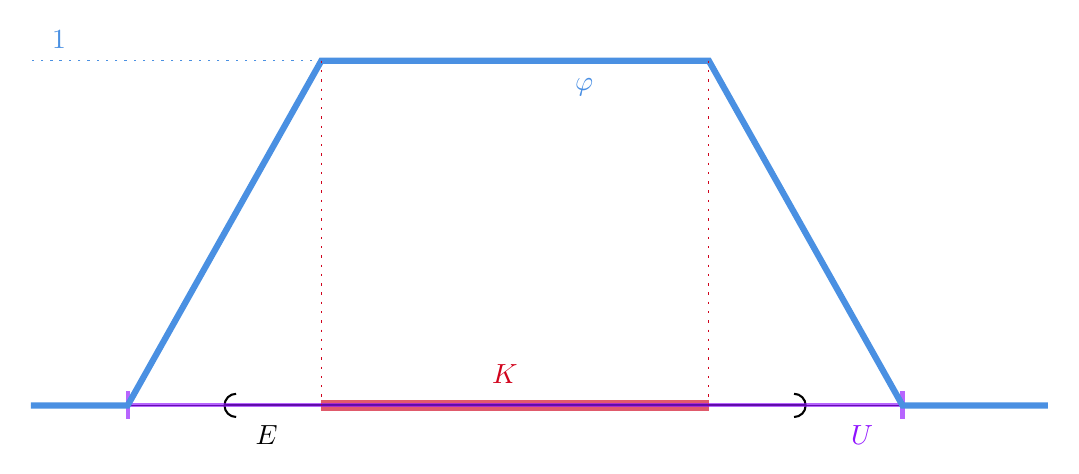
\begin{tikzpicture}[x=0.75pt,y=0.75pt,yscale=-1,xscale=1]
%uncomment if require: \path (0,300); %set diagram left start at 0, and has height of 300

%Straight Lines [id:da3965910987726231] 
\draw    (20,230.72) -- (510,230.72) ;
%Straight Lines [id:da4009915020269945] 
\draw [color={rgb, 255:red, 208; green, 2; blue, 27 }  ,draw opacity=0.65 ][fill={rgb, 255:red, 208; green, 2; blue, 27 }  ,fill opacity=1 ][line width=3.75]    (160,230.72) -- (346.67,230.72) ;
%Straight Lines [id:da44297607097165415] 
\draw [line width=0.75]    (113.33,230.72) -- (393.33,230.72) ;
\draw [shift={(393.33,230.72)}, rotate = 180] [color={rgb, 255:red, 0; green, 0; blue, 0 }  ][line width=0.75]      (5.59,-5.59) .. controls (2.5,-5.59) and (0,-3.09) .. (0,0) .. controls (0,3.09) and (2.5,5.59) .. (5.59,5.59) ;
\draw [shift={(113.33,230.72)}, rotate = 0] [color={rgb, 255:red, 0; green, 0; blue, 0 }  ][line width=0.75]      (5.59,-5.59) .. controls (2.5,-5.59) and (0,-3.09) .. (0,0) .. controls (0,3.09) and (2.5,5.59) .. (5.59,5.59) ;
%Straight Lines [id:da09002804097538131] 
\draw [color={rgb, 255:red, 144; green, 19; blue, 254 }  ,draw opacity=0.65 ][fill={rgb, 255:red, 144; green, 19; blue, 254 }  ,fill opacity=1 ][line width=1.5]    (66.67,230.72) -- (440,230.72) ;
\draw [shift={(440,230.72)}, rotate = 180] [color={rgb, 255:red, 144; green, 19; blue, 254 }  ,draw opacity=0.65 ][line width=1.5]    (0,6.71) -- (0,-6.71)   ;
\draw [shift={(66.67,230.72)}, rotate = 180] [color={rgb, 255:red, 144; green, 19; blue, 254 }  ,draw opacity=0.65 ][line width=1.5]    (0,6.71) -- (0,-6.71)   ;
%Straight Lines [id:da8673358856748661] 
\draw [color={rgb, 255:red, 74; green, 144; blue, 226 }  ,draw opacity=1 ][line width=2.25]    (20,230.72) -- (66.67,230.72) -- (160,64.64) -- (346.67,64.64) -- (440,230.72) -- (510,230.72) ;
%Straight Lines [id:da7029234521695775] 
\draw [color={rgb, 255:red, 74; green, 144; blue, 226 }  ,draw opacity=1 ] [dash pattern={on 0.84pt off 2.51pt}]  (160,64.64) -- (20,64.64) ;
%Straight Lines [id:da15474017698585407] 
\draw [color={rgb, 255:red, 208; green, 2; blue, 27 }  ,draw opacity=1 ] [dash pattern={on 0.84pt off 2.51pt}]  (160,64.64) -- (160,230.72) ;
%Straight Lines [id:da9821160247046214] 
\draw [color={rgb, 255:red, 208; green, 2; blue, 27 }  ,draw opacity=1 ] [dash pattern={on 0.84pt off 2.51pt}]  (346.67,64.64) -- (346.67,230.72) ;

% Text Node
\draw (127,239) node [anchor=north west][inner sep=0.75pt]   [align=left] {$\displaystyle E$};
% Text Node
\draw (241,210) node [anchor=north west][inner sep=0.75pt]   [align=left] {$\displaystyle \textcolor[rgb]{0.82,0.01,0.11}{K}$};
% Text Node
\draw (414,239) node [anchor=north west][inner sep=0.75pt]   [align=left] {$\displaystyle \textcolor[rgb]{0.56,0.07,1}{U}$};
% Text Node
\draw (29,49) node [anchor=north west][inner sep=0.75pt]  [color={rgb, 255:red, 74; green, 144; blue, 226 }  ,opacity=1 ] [align=left] {$\displaystyle 1$};
% Text Node
\draw (281,72) node [anchor=north west][inner sep=0.75pt]   [align=left] {$\displaystyle \textcolor[rgb]{0.29,0.56,0.89}{\varphi }$};


\end{tikzpicture}

            \caption{Построение $\varphi$.}
            \label{fig:lect14:kp}
        \end{figure}

        Более формально,
        возьмем функцию $\psi(x)=\rho(x,\, K)$, из математического анализа известно, что
        она непрерывна.
        Видно, что подойдет функция \[
            \varphi(x)=\dfrac{\rho(x,\, U^C)}{\rho(x,\, K)+\rho(x,\, U^C)}
        \]
        Итак, $\varphi$~--- непрерывна и равна 0 на $U^C$, следовательно она финитна.
        Далее \[
            0\leqslant \varphi\leqslant1,\quad \varphi(K)=1\Rightarrow
            \int |1_E-\varphi|d\lambda=\int_{U\setminus K}|\varphi|d\lambda\leqslant
            \lambda(U\setminus K)<\varepsilon.
        \]

    \end{proof}
\end{claim}

\begin{remark}
    Легко понять, что данное доказательство обобщается на случай $\R^d,\, d\in\N$.
\end{remark}

\begin{theorem}[лемма Римана-Лебега]
    Если $f\in L^1(\R)$, то \[
        \lim_{n\toi}\int f(x)\cdot \sin(nx)dx=0.
    \]

    \begin{proof}

        Пусть $\varepsilon>0$, тогда существует финитная функция $\varphi\in C_c(\R)$, которая
        приближает $f$: $\|f-\varphi\|_1<\varepsilon$. Тогда \[
            \left|\int f\sin(nx)dx\right|\leqslant\int |f-\varphi|\sin (nx)dx+
            \left|\int \varphi\sin (nx)dx\right|
        \]
        Первый интеграл ограничен сверху $\varepsilon$.
        Второй интеграл можно рассматривать в смысле Римана (по доказанному ранее в силу непрерывности),
        а в курсе математического анализа было доказано, что \[
            \lim_{n\toi}\int \varphi\sin(nx)dx=0.
        \]

    \end{proof}
\end{theorem}

\begin{exercise}
    Можно ли из последовательности $f_n(x)=\sin nx$ выделить подпоследовательность,
    сходящуюся почти всюду (относительно меры Лебега)?

    \textbf{Ответ:} нет.

    \textbf{Указание.} Если $\sin n_kx\to f(x)$ п. в., то $f(x)\sin n_kx\to f^2(x)$ п. в.
    Далее нужно рассмотреть $\int_0^1 f^2(x)dx$.
\end{exercise}

\begin{claim}[1-ая лемма Бореля-Кантелли]
    Рассмотрим пространство с мерой: $(X,\, \CE,\, \mu)$.
    Пусть дана последовательность множеств $\{E_k\}_{k\in\N}\subset\CE$
    причем $\sum\limits_{k=1}^{\infty}\mu(E_k)<\infty$.

    Тогда $\mu$"=п. в. $x$ принадлежат не более чем конечному набору множеств $E_k$,
    то есть \[
        \exists N\in\CE:\quad \mu(N)=0\quad \forall x\in N^C\quad
        \exists n=n(x)\in \N:\quad \forall k\geqslant n:\quad   x\notin E_k.
    \]

    \begin{proof}

        Пусть \[
            f(x):=\sum_{k=1}^{\infty}1_{E_k}(x).
        \]
        Тогда по теореме о монотонной сходимости\[
            \int f(x)d\mu=\sum_{k=1}^{\infty}\mu(E_k)<\infty\Rightarrow f\in L^1\Rightarrow
            f\text{~--- конечна $\mu$"=п. в.}
        \]
        Поэтому \[
            \exists N\in\CE:\quad \mu(N)=0\quad\forall x\in N^C\quad f(x)<\infty
            \Rightarrow\sum_{k=1}^{\infty}1_{E_k}(x)<\infty
        \]
        А значит, \[
            \{k\in\N:\: x\in E_k\}\text{~--- конечно,}
        \]
        потому что мощность данного множества и является конечной суммой выше.

    \end{proof}
\end{claim}

\subsection{Сходимость по мере.}

\begin{definition}
    Если $\{f_n\}_n$ и $f$ измеримы относительно $\CE$, то будем говорить, что
    $f_n$ \mdef{сходится} к $f$ по мере при $n\toi$ (обозначение:
    $f_n\xrightarrow[n\toi]{\mu}f$), если \[
        \forall \varepsilon>0\quad \mu\left(\underbrace{\{x\in X:\: |f_n(x)-f(x)|>\varepsilon\}}_{\in\CE}
        \right)
        \xrightarrow[n\toi]{}0.
    \]
\end{definition}

\begin{claim}
    Пусть $\mu$~--- конечна. Тогда \begin{enumerate}
        \item Если $f_n\to f$ $\mu$"=п. в., то $f_n\xrightarrow[]{\mu}f$.
        \item Если $f_n\to f$ в $L^1$, то $f_n\xrightarrow[]{\mu}f$.
    \end{enumerate}

    \begin{proof}

        \begin{enumerate}
            \item Для начала перепишем меру:\[
                      \mu\left(\{x\in X:\: |f_n(x)-f(x)|>\varepsilon\}\right)=\int 1_{\{|f_n-f|>\varepsilon\}}(x)d\mu(x).
                  \]
                  Пусть $\varepsilon>0$.
                  Итак, $f_n\to f$ $\mu$"=п. в., тогда для $\mu$"=п. в. $x$ при достаточно больших $n$:
                  \[
                      |f_n(x)-f(x)|<\varepsilon\Rightarrow 1_{\{|f_n-f|>\varepsilon\}}(x)=0\Rightarrow
                      1_{\{|f_n-f|>\varepsilon\}}\xrightarrow[n\toi]{}0\text{ $\mu$"=п. в.}
                  \]
                  Далее, \[
                      1_{\{|f_n-f|>\varepsilon\}}\leqslant 1\in L^1,
                  \]
                  так как $\int 1d\mu=\mu(X)<\infty$.
                  Следовательно, по теореме Лебега \[
                      \int 1_{1_{\{|f_n-f|>\varepsilon\}}}d\mu\xrightarrow[n\toi]{}0.
                  \]

            \item Пусть $\varepsilon>0$. В силу неравенства Чебышева \[
                      \mu\left(\{|f_n-f|>\varepsilon\}\right)\leqslant\dfrac{1}{\varepsilon}
                      \int |f_n-f|d\mu\xrightarrow[n\toi]{}0.
                  \]
        \end{enumerate}

    \end{proof}
\end{claim}

\begin{remark}
    Из сходимости по мере не следует сходимость почти всюду и сходимость в среднем.
\end{remark}

\begin{theorem}[Рисс]
    Если $f_n\to f$ по мере, то $\exists\{f_{n_k}\}:\: f_{n_k}\to f$ $\mu$"=п. в.

    \begin{proof}

        Рассмотрим множество \[
            A_n^{\varepsilon}:=\{x\in X:\: |f_n(x)-f(x)|\geqslant\varepsilon\}.
        \]
        Для любого фиксированного $\varepsilon>0$ по определению сходимости по мере
        $\mu(A_n^{\varepsilon})\xrightarrow[n\toi]{}0$.
        Будем брать $\varepsilon=\dfrac{1}{k}$, тогда $\exists n=n_k:\:\mu(\underbrace{A_{n_k}^{1/k}}_{E_k})<2^{-k}$.
        Тогда $\sum_{k=1}^{\infty}\mu(E_k)<\infty$, поэтому для $\mu$"=п. в. $x$ существует
        $n=n(x)$ такое, что при $k>n\ x\notin E_k$, следовательно \[
            |f_k(x)-f(x)|<\dfrac{1}{k}\xrightarrow[k\toi]{}0
            \Rightarrow f_k(x)\xrightarrow[k\toi]{}f(x).
        \]

    \end{proof}
\end{theorem}

\begin{theorem}[Егоров]
    Пусть $\mu(X)<\infty$.
    Если $f_n\to f$ $\mu$"=п. в., то \[
        \forall \varepsilon>0\quad \exists N\in\CE:\quad
        \mu(N)<\varepsilon:\quad f_n\xrightrightarrows[N^C]{} f\text{ при } n\toi.
    \]
\end{theorem}